%!TEX root = ../thesis-main.tex
\chapter{Analisi}

\section{Requisiti}

Il progetto si pone due principali obiettivi:
\begin{itemize}
	\setlength\itemsep{0.8em}
	\item La generazione automatica di pacchetti di installazione multi-piattaforma \\ con \ac{jre} integrato
	\item La pubblicazione automatica dei rilasci del software all'interno di repository pubblici selezionati
\end{itemize}
Con integrazione di un \ac{jre} si intende il supplemento di una \ac{jvm} all'interno del pacchetto di installazione.
L'utente potrebbe non aver alcun \ac{jre} installato sul proprio dispositivo, oppure quello presente potrebbe essere obsoleto. Inserendo una macchina virtuale Java: si fornisce uno specifico ambiente di esecuzione eliminando potenziali problemi di compatibilità e si agevola la procedura di installazione per l'utente finale.

\paragraph{Requisiti funzionali}

Le funzionalità richieste si possono classificare in due gruppi distinti: il primo contiene tutto ciò che concerne l'esperienza dell'utente finale, mentre il secondo descrive le funzionalità dal punto di vista degli sviluppatori e contributori di Alchemist. Di seguito il primo gruppo:
\begin{itemize}
	\item \textbf{Pacchettizzazione}: il simulatore deve essere distribuito in pacchetti auto-contenuti, ossia comprendenti di tutto il necessario per l'utilizzo di esso.
	\item \textbf{Multi-piattaforma}: Alchemist deve essere installabile sui maggiori sistemi operativi in circolazione come Windows, MacOS e le principali distribuzioni Linux.
	\item \textbf{Pronto all'uso}: l'installazione non deve richiedere configurazioni complesse, l'applicativo deve essere pronto all'uso non appena installato.
\end{itemize}

I requisiti del gruppo successivo sono accumunabili per il loro scopo, vale a dire l'automazione.

\begin{itemize}
	\item \textbf{Automazione dei pacchetti}: la generazione dei pacchetti di installazione deve essere automatica e configurabile
	\item \textbf{Automazione della distribuzione}: il rilascio di una nuova versione deve essere eseguito interamente in automatico, compreso la distribuzione nei repository selezionati.
	\item \textbf{Verifica funzionamento}: entrambi i processi descritti precedentemente devono essere corredati da verifiche del loro funzionamento e devono bloccare la procedura di rilascio nell'eventualità siano presenti errori.
\end{itemize}

\paragraph{Requisiti non funzionali}

\begin{itemize}
	\item Trattandosi Alchemist di un software in continuo sviluppo, è auspicabile l'utilizzo degli strumenti già impiegati all'interno del repository. \\ L'integrazione di nuovi applicativi deve essere eseguita solo se strettamente necessaria.
	\item La pipeline \ac{cicd} ottenuta deve garantire prestazioni in linea con la versione precedente l'intervento di questo progetto.
\end{itemize}

\section{Pacchettizzazione}\label{sec:packaging}

Come si evince dall'analisi svolta, la pacchettizzazione è requisito fondamentale dell'elaborato. Sino ad ora l'applicativo Alchemist era distribuito in file JAR, ossia archivi java compressi contenenti tutte le dipendenze ed i relativi \textit{classfiles} necessari all'esecuzione. Quest'approccio molto diffuso porta con sè diverse limitazioni tra cui:
\begin{itemize}
	\item la necessità dell'utente scaricante di avere un \ac{jre} installato nel proprio dispositivo,
	\item il potenziale bisogno di utilizzare un ambiente \ac{jre} specifico e quindi per l'utente di non possedere una versione dell'ambiente compatibile,
	\item la difficoltà di utilizzo per utenti non esperti, i quali sono abituati ad eseguire programmi utilizzando file eseguibili nativi della propria piattaforma.
\end{itemize}

Seppur alcune di queste restrizioni sono in parte mitigate in certe piattaforme, non è lo stesso per altre molto diffuse come Windows, il quale per esempio non fornisce un ambiente java pre-installato. Esistono diversi strumenti di terze parti e non che cercano di far fronte a questo problema, è importante dunque valutare e scegliere lo strumento più opportuno.

\subsection{Soluzioni}

Nell'ottica di semplificare la configurazione di questo processo lo strumento selezionato deve supportare le tre principali piattaforme descritte nei requisiti precedentemente. Tra gli strumenti analizzati due molto differenti si sono distinti, vale a dire: \textit{jpackage}, comando disponibile nel \ac{jdk} dalla versione 14 adibito alla produzione di pacchetti auto-contenuti con \ac{jre} integrata e \textit{GraalVM}, un \ac{jdk} sviluppato da Oracle che fornisce un compilatore \ac{jit} e \ac{aot} per java. Il termine \ac{jit} descrive il comportamento normale di ogni \ac{jvm}: il \textit{java compiler} traduce il programma ad alto livello in \textit{bytecode}, successivamente la \ac{jvm} trasforma il bytecode in linguaggio macchina specifico per l'architettura sottostante eseguendo dunque una compilazione dinamica. In contrasto la tecnica \ac{aot} ricorda i linguaggi di programmazione compilati, la compilazione è statica ed avviene prima dell'esecuzione del programma. Il compilatore \ac{aot} chiamato ``Native Image", consente di compilare un programma java (ed altri linguaggi di programmazione) ottenendo in output un eseguibile nativo per ogni piattaforma. Quest'ultimo inoltre porta con sè diversi vantaggi come: un minor costo in risorse CPU e memoria, tempi di avvio minori e dimensioni ridotte rispetto un normale programma java distribuito con un \ac{jre}. L'annessione di un JRE non è quindi necessaria, l'eseguibile prodotto contiene tutto il necessario per l'esecuzione dell'applicazione, eliminando la necessità di una macchina virtuale java. La compilazione \ac{aot} però ha dei requisiti, uno di questi fondamentale è la \textit{closed world assumption}: ossia ogni parte di codice raggiungibile in esecuzione lo deve essere anche in fase di build, altrimenti quei componenti non appariranno nell'eseguibile finale. Ciò accade perché native image svolge un analisi statica del codice e dunque non lo esegue, alcune funzionalità come la reflection oppure il caricamento dinamico non sono supportate e richiedono una soluzione alternativa.

In contrasto jpackage fornisce uno strumento interessante, il quale non richiede modifiche all'applicativo e si trova pre-installato in tutti i \ac{jdk} dalla versione 14 in poi. Supporta nativamente l'annessione di un \ac{jre} utilizzando \textit{jlink}, produce diverse tipologie di pacchetti per ogni piattaforma ed è completamente controllabile da interfaccia \ac{cli}: particolare molto d'aiuto nei successivi step di automazione. Le tipologie di pacchetti generabili sono elencati di seguito:
\begin{itemize}
	\item EXE e MSI per Windows
	\item RPM e DEB per Linux
	\item PKG e DMG per MacOs.
\end{itemize}
Anch'esso presenta dei limiti come: la necessità di essere eseguito sullo stesso sistema operativo dove i pacchetti prodotti sono destinati (lo stesso vale per GraalVM, la \textit{cross compilation} non è supportata) e la produzione di un solo pacchetto ad ogni esecuzione.

\paragraph{Valutazione finale} Ambedue le soluzioni concorrono all'obiettivo primario, la distribuzione del software multi-piattaforma e pronto all'uso. GraalVM fornisce diversi vantaggi prestazionali, ma i requisiti da esso richiesti non sono compatibili con l'architettura del simulatore. D'altro canto jpackage fornisce tutto il necessario per costruire i pacchetti con embed di un \ac{jre} e i limiti delineati sono superabili adoperando script o configurazioni specifiche.

\section{Strumenti}

\subsection{Gradle}

Mentre in passato la produzione di artefatti (documentazione, pacchetti, eseguibili) era delegata a script costruiti dallo sviluppatore, in un progetto di grandi dimensioni è oggigiorno essenziale avvalersi di uno strumento di build automation. Come l'output di un programma deterministico non cambia per uno stesso input, la produzione di artefatti deve essere consistente e riproducibile riducendo al minimo l'intervento umano. 

Gradle è uno dei tanti strumenti disponibili, supporta diversi linguaggi di programmazione anche se risulta popolare nell'ambiente JVM come alternativa a Maven. I \textit{task} sono l'unità minima di esecuzione e rappresentano un azione: come generare un JAR, eseguire dei test o produrre la documentazione. Mediante direttive come \textit{dependsOn} è possibile creare dipendenze tra processi, Gradle per orchestrare l'esecuzione dei task costruisce un grafo aciclico diretto (DAG) delle dipendenze. L'esecuzione di Gradle avviene in tre fasi distinte elencate di seguito.
\begin{enumerate}
	\item \textbf{Fase di inizializzazione}. In primo luogo Gradle crea un'istanza di Settings che organizza l'architettura del progetto. Attraverso un file, di nome ``settings.gradle", lo sviluppatore stabilisce il progetto radice e tutti gli eventuali progetti figli. 
	\item \textbf{Fase di configurazione}. Successivamente tutti i file di configurazione ``build.gradle" (del progetto radice e tutti i sotto-progetti) vengono analizzati per costruire il grafo dei task.
	\item \textbf{Fase di esecuzione}. Infine, Gradle esegue i task richiesti considerando le dipendenze descritte nel grafo generato nella fase precedente.
\end{enumerate}

\begin{figure}[htb]
	\centering
	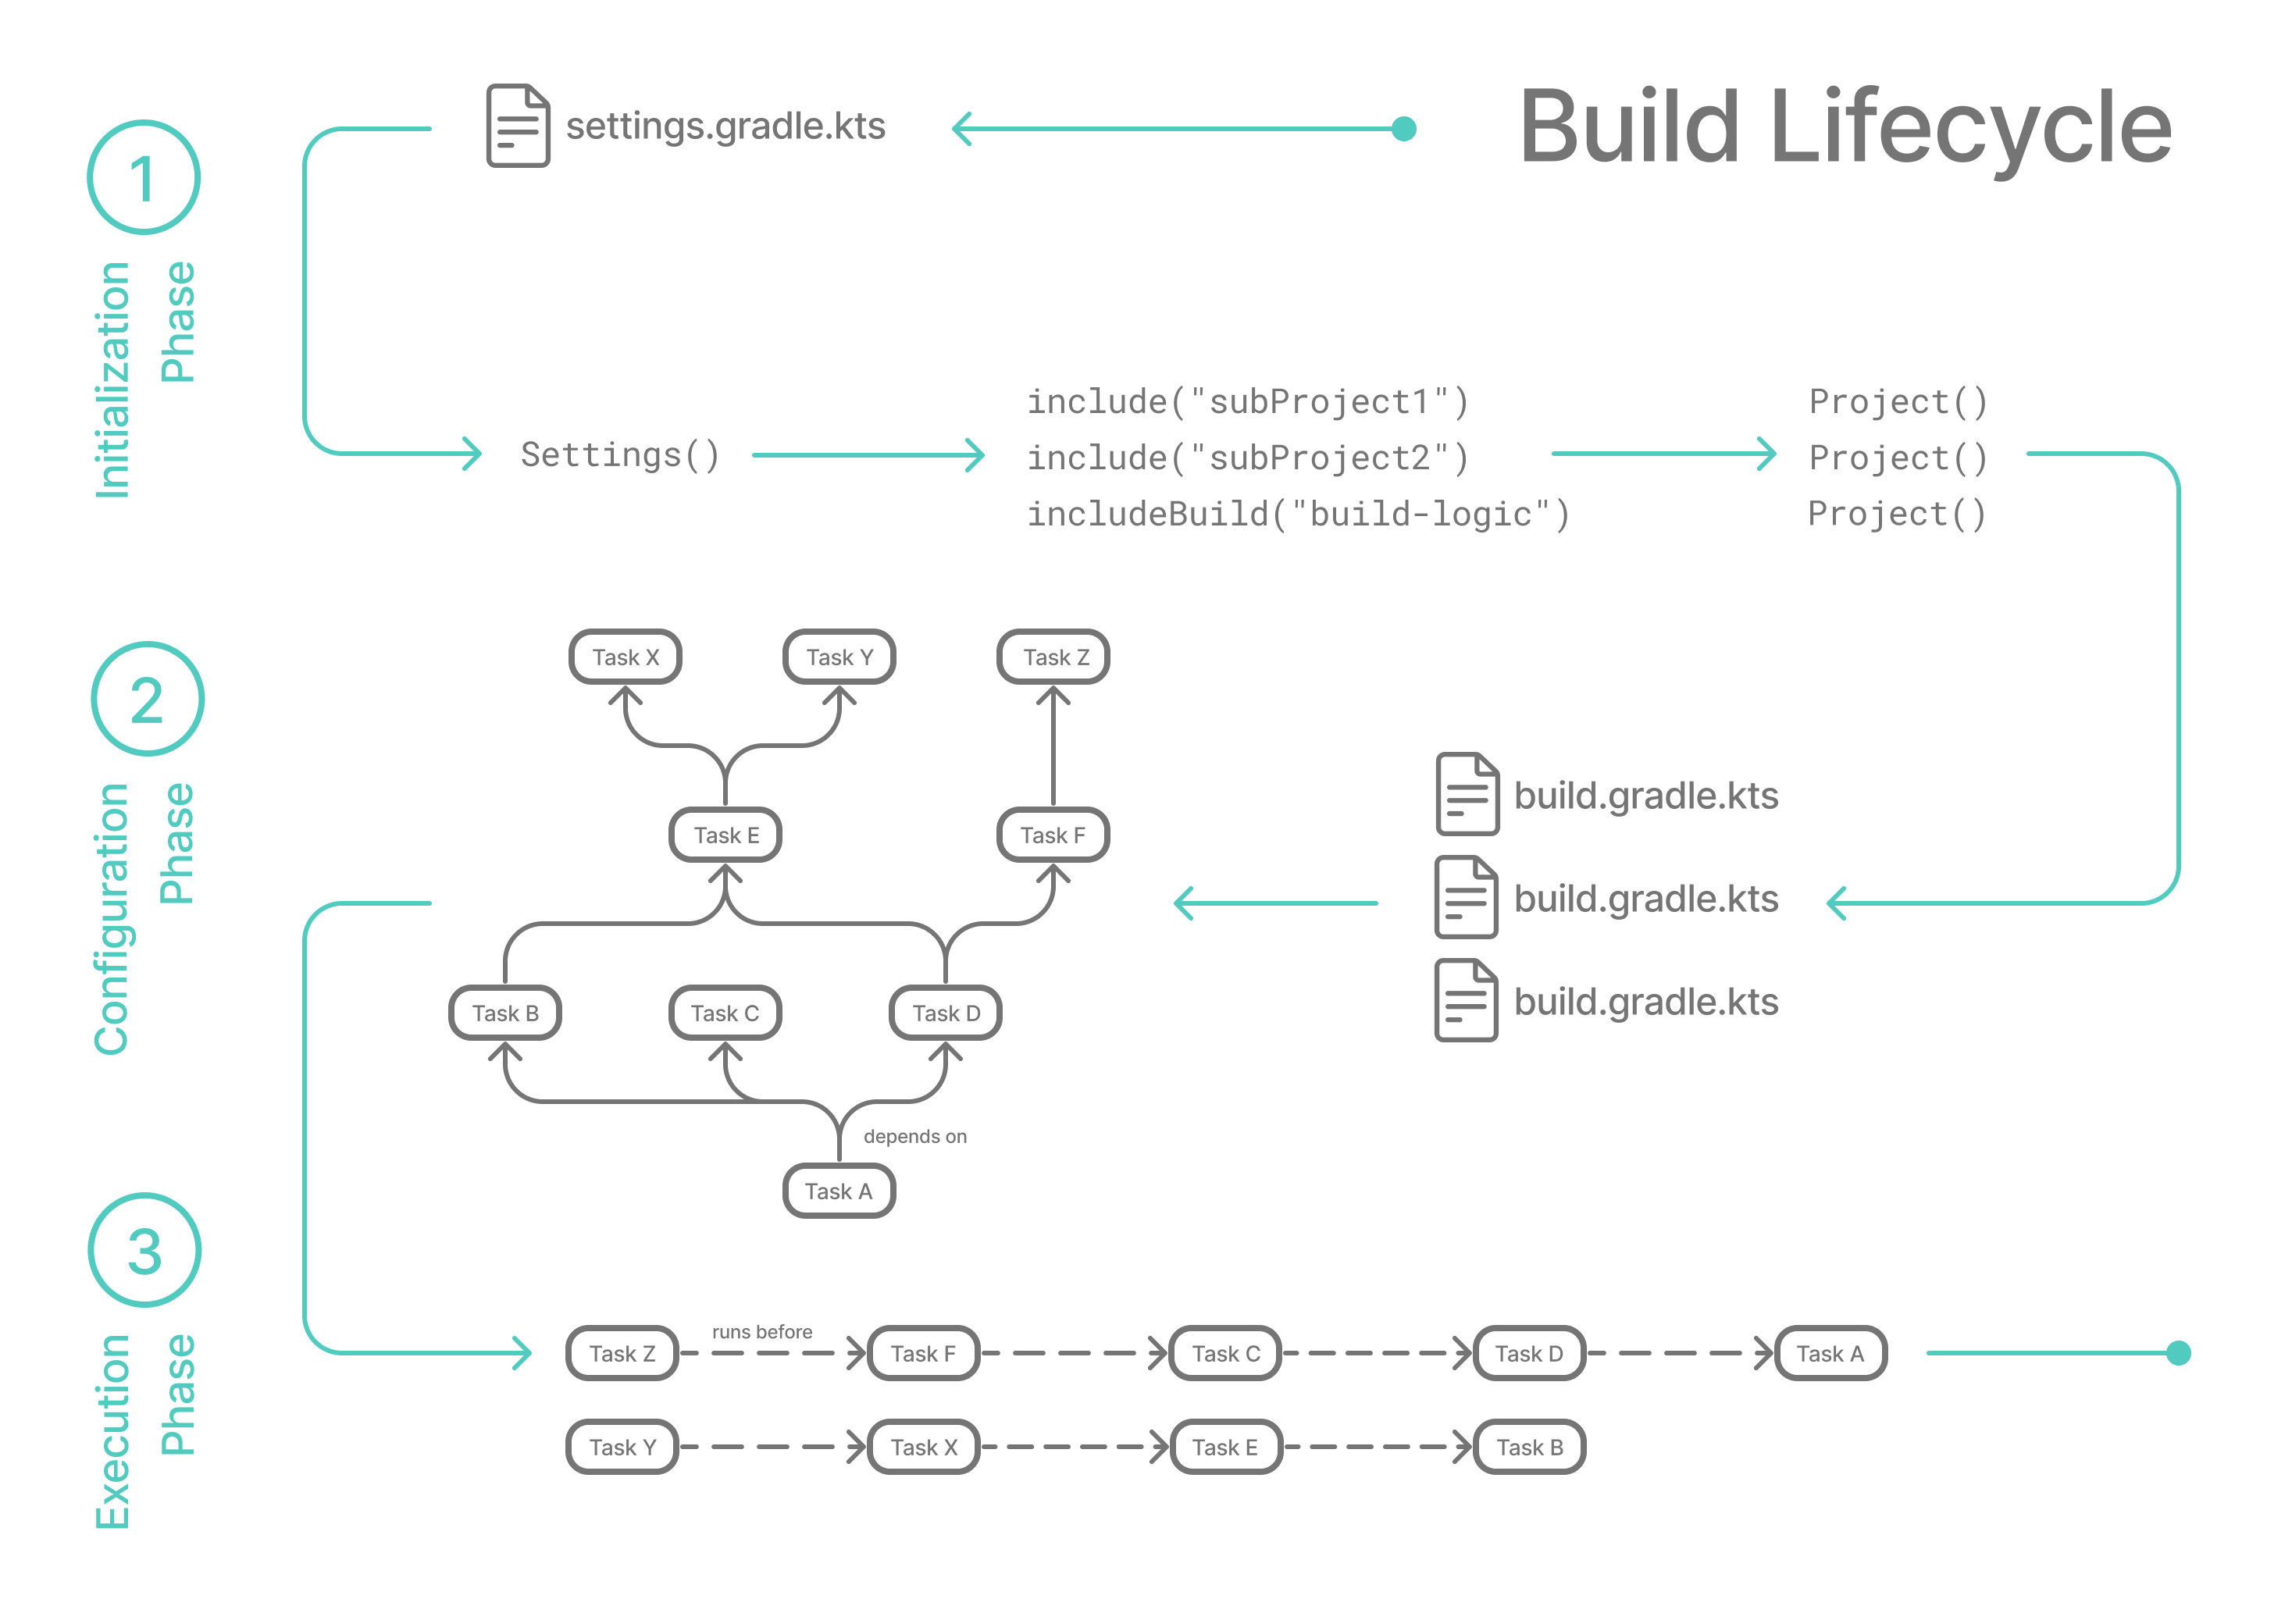
\includegraphics[width=.9\linewidth]{figures/gradle-build-lifecycle-example.png}
	\caption{Esempio di inizializzazione, configurazione ed esecuzione di una build Gradle}
	\label{fig:gradle-build-lifecycle}
\end{figure}

Un componente chiave sono i plugin, i quali consentono di estendere le funzionalità di Gradle: aggiungere nuovi task, estendere il modello con nuovi elementi ed applicare configurazioni specifiche all'intero progetto. La presenza di diversi plugin base e creati dalla comunità rende Gradle uno strumento versatile.

\paragraph{Analisi rispetto ai requisiti}
In considerazione dei requisiti di automazione, Gradle fornisce le funzionalità necessarie a soddisfare i requisiti di pacchettizzazione, distribuzione e verifica del funzionamento. Utilizzando Gradle si integrano questi processi all'interno del build system garantendo un corretto ordine di esecuzione con l'effetto di minimizzare l'incidenza di errori e assicurando la produzione di pacchetti conformi su qualsiasi sistema operativo questo venga eseguito.
L'approccio orientato ai task inoltre permette di suddividere un macro-processo in più unità di esecuzione riutilizzabili da altri processi, garantendo tutti i vantaggi che la filosofia \ac{dry} fornisce.

\subsection{GitHub Actions}

Tramite Gradle lo sviluppatore è in grado di eseguire procedure articolate come compilazione, test e dispiegamento utilizzando un semplice comando da \ac{cli}. L'e\-se\-cu\-zio\-ne di queste procedure richiede però l'intervento umano, è quindi necessario uno strumento capace di automatizzare queste procedure offrendo un infrastruttura resiliente e facilmente accessibile.

GitHub Actions è una piattaforma per automatizzare processi di \ac{cicd} disponibile per i repository ospitati su GitHub. Gli sviluppatori utilizzano esso per eseguire automaticamente test ad ogni commit, controllare il codice fornito dai contributori o distribuire regolarmente l'applicazione. Consente la configurazione ed esecuzione di pipeline personalizzate, ovvero i \textit{workflow} processi eseguibili consistenti in un insieme di \textit{job} eseguiti sequenzialmente o parallelamente all'interno di macchine virtuali dette \textit{runner}. I workflow vengono eseguiti quando un certo evento, configurato dallo sviluppatore, si manifesta. GitHub in primo luogo è una piattaforma di code-sharing orientata allo sviluppo open source, una peculiarità della funzionalità Actions è la vasta gamma di eventi legati alla piattaforma: dall'apertura di una pull-request, un commento o la creazione di un fork.

I workflow (figura \ref{fig:github-actions-example}) sono descritti in file YAML all'interno di una cartella specifica del repository. In primis si configura il nome del workflow e l'evento che origina l'esecuzione di esso, successivamente l'elenco dei job e gli step, l'unità di esecuzione minima che raggruppate modellano l'azione svolta dal job.

\begin{figure}[htb]
	\centering
	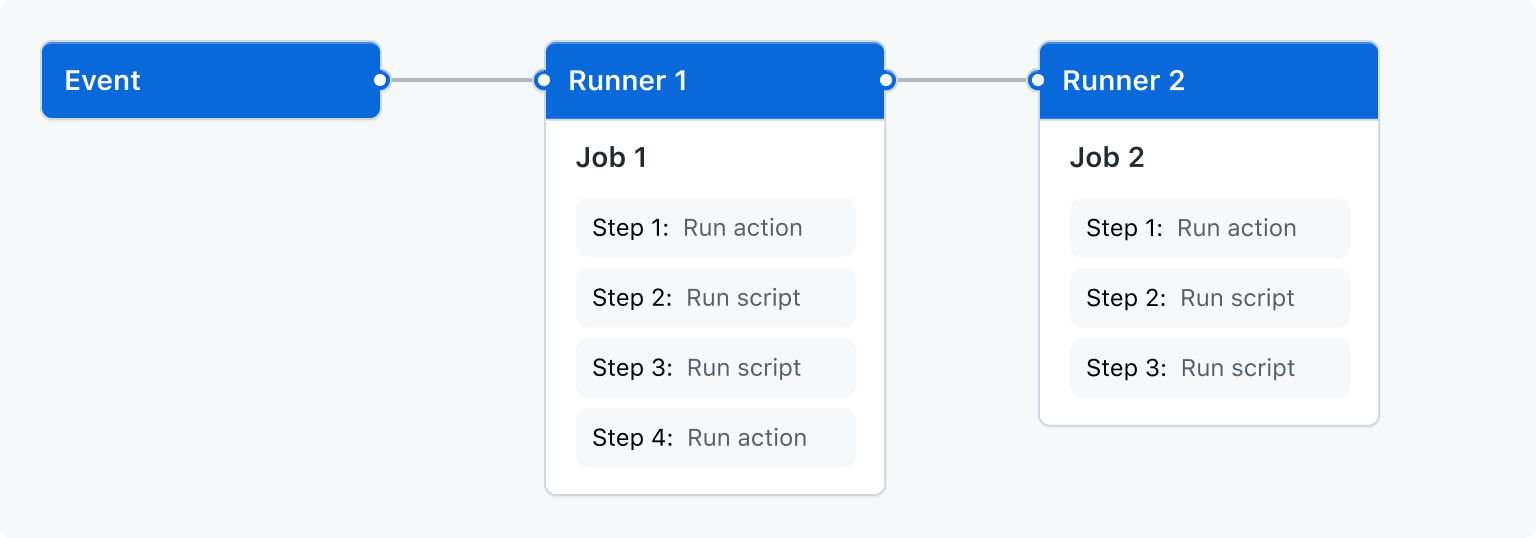
\includegraphics[width=.9\linewidth]{figures/overview-actions-simple.png}
	\caption{Sintesi dei componenti utilizzati su GitHub Actions ed esempio di un workflow \\ source: https://docs.github.com/en/actions/learn-github-actions/understanding-github-actions}
	\label{fig:github-actions-example}
\end{figure}

Uno step può presentare una lista di comandi eseguiti nella shell di riferimento (quella di default per il sistema operativo o un'altra se specificata) altrimenti un'\textit{action}. Le action sono componenti riutilizzabili che eseguono un'attività precisa, esistono diverse azioni sviluppate dalla comunità e rese disponibili all'interno di un marketplace vasto. Per esempio una delle più diffuse ed utilizzate è ``actions/checkout" [\cite{github-actions-diffusion}], la quale clona il repository del progetto nella cartella di lavoro corrente del runner.

\paragraph{Analisi rispetto ai requisiti}

La piattaforma di GitHub Actions ricopre un ruolo fondamentale: offre l'infrastruttura per l'e\-se\-cu\-zio\-ne dei processi quali vogliamo automatizzare. Rispetto ai requisiti risponde con successo presentando:
\begin{itemize}
	\item la possibilità di utilizzare macchine virtuali (runner) di tutte e tre i sistemi operativi target,
	\item la possibilità di configurare eventi o esecuzioni ricorrenti del processo costruito, assicurando quindi l'automazione di quest'ultimo.
\end{itemize}
Riguardo invece i requisti non funzionali, il workflow deve sfruttare le funzionalità di Actions per ottimizzare l'esecuzione del flusso, riducendo i tempi di sviluppo e i costi collegati all'utilizzo della piattaforma.

\subsection{Package manager}

Nei sistemi operativi Linux il controllo dei componenti installati nella macchina è completamente delegato ai \textit{package manager}. Il \textit{package-management system} è un insieme di strumenti software che gestiscono i processi di installazione, aggiornamento, configurazione e rimozione di applicativi dal sistema. Spesso un pacchetto corrisponde ad un particolare programma o applicazione, contemporaneamente però esistono applicativi più complessi composti da numerosi pacchetti correlati. Il sistema di gestione dei pacchetti opera attraverso tre componenti principali.

\begin{itemize}
	\item Un componente a basso livello che si occupa principalmente dell'installazione o rimozione dei pacchetti. Definito come il back-end dei package-management system, è il caso di \textbf{rpm} il quale gestisce gli omonimi pacchetti e dpkg per i pacchetti \textbf{deb}.
	\item Un componente ad alto livello il cui compito principale è quello di fornire un'interfaccia all'utente come: \textbf{yum} per Fedora o \textbf{apt} per Debian. Si occupa inoltre di risolvere le dipendenze e gestire le sorgenti esterne (repository).
	\item I repository, ossia database pubblici ufficiali o no contenenti i pacchetti ed i relativi meta-dati.
\end{itemize}

\begin{figure}[H]
	\centering
	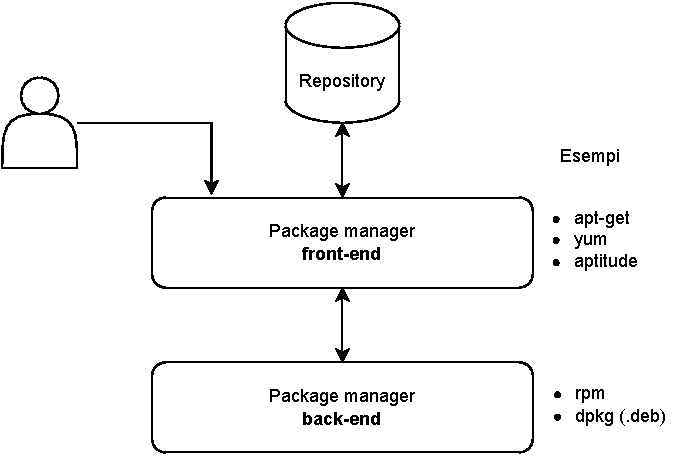
\includegraphics[width=.7\linewidth]{figures/package-managers.pdf}
	\caption{Struttura più diffusa dei sistemi di gestione di pacchetti}
	\label{fig:package-managers}
\end{figure}

\paragraph{Arch User Repository} Una distribuzione importante nel vasto panorama dei fork Linux è Arch. Arch è una distribuzione Linux con architettura x86-64 creata seguendo la filosofia \ac{kiss}. È infatti rinomata per essere leggera, veloce, estremamente scalabile ed adattabile alle proprie esigenze. Data la sua natura minimalista, l'installazione iniziale non incorpora alcun strumento di configurazione automatica, nessun ambiente desktop e nessun altro strumento necessario all'avvio del sistema. Il sistema di gestione dei pacchetti si chiama \textit{pacman} ed a differenza dei concorrenti, opera sia a basso che ad alto livello. Un pacchetto non è altro che un file shell script denominato \textit{PKGBUILD} contenente le istruzioni necessarie a scaricare i sorgenti e compilarli attraverso un comando: \textit{makepkg}. La linearità dei file PKGBUILD rende la creazione di pacchetti alla portata di qualsiasi utente difatti Arch supporta \textbf{\ac{aur}}, un tratto distintivo di questa distribuzione. Si tratta di un repository di pacchetti in cui qualsiasi utente, anche non sviluppatore, può contribuire.  

\paragraph{Windows e winget} Nell'ambiente Windows fino a poco tempo fa non prevedeva alcun package manager ufficiale pre-installato. Solamente dal settembre 2020 è nato ``winget": package-management system open-source sviluppato da Microsoft. Supporta pacchetti di installazione EXE, MSIX e MSI. Il repository dei pacchetti è accessibile pubblicamente ed è possibile mediante richieste di contribuzione e previa approvazione, pubblicare pacchetti all'interno di esso.

\paragraph{Pacchetti containerizzati} Un'altra tipologia sono i pacchetti detti containerizzati, ovvero eseguiti all'interno di ambienti separati dal sistema. Questa caratteristica fornisce due principali vantaggi: la possibilità per una applicazione di usare la propria versione desiderata di librerie di sistema senza creare conflitti e la trasparenza all'utente nell'accesso di risorse di sistema, garantendo un livello di sicurezza maggiore rispetto pacchetti gestiti normalmente.

\paragraph{Analisi rispetto ai requisiti}
Nell'ottica di soddisfare il requisito multi-piattaforma del progetto è necessario analizzare le piattaforme di destinazione per il simulatore. Mentre per Windows e MacOS esistono specifiche tipologie di pacchetti di installazione supportati ufficialmente, per Linux non esiste uno standard univoco. Tuttavia  i pacchetti RPM e DEB sono supportati dalla maggior parte delle distribuzioni, in particolare il primo è citato nella specifica ``Linux Standard Base". Il PKGBUILD di Arch supporta nativamente l'estrazione di sorgenti RPM e DEB, pertanto a fronte di questa analisi essi risultano la scelta più opportuna.
